\documentclass[11pt]{article}

\usepackage[margin=1in]{geometry}
\usepackage[T1]{fontenc}
\usepackage{amsmath}
\usepackage{amssymb}
\usepackage{graphicx}
\usepackage{booktabs}
\usepackage{verbatim}
\usepackage{hyperref}
\usepackage{url}

\setlength{\emergencystretch}{3em}   % avoid overfull lines around long file names
\setlength{\parskip}{0.4em}
\setlength{\parindent}{0pt}

\newcommand{\code}[1]{\texttt{#1}}

\title{\vspace{-2em}COMP626: Applied Math for Scientists - Project 1\\[0.3em]
\large The Pleiades Problem}
\author{Annice Najafi}
\date{}

\begin{document}
\maketitle
\vspace{-3em}

\section{Introduction: the Pleiades before the differential equation}

Long before the development of telescopes or modern astronomy, humans
learned about the sky simply by watching it \cite{thurston1994early}. Generation after generation
observed that particular stars appeared and disappeared at predictable times of
the year and they learned to rely on the night sky as a natural calendar for agriculture, migration,
navigation and seasonal change \cite{edgar2019observer}. Among the most conspicuous objects in this
ancient sky was a small, tightly packed group of stars which is now known as the
Pleiades, or Messier 45 (M45). Located in the constellation Taurus
approximately 445 light-years from Earth, the Pleiades is actually an open
cluster containing more than a thousand stars, although only a small number are
bright enough to dominate its appearance to the unaided human eye
\cite{nasa-m45}.

\begin{figure}[htbp]
\centering
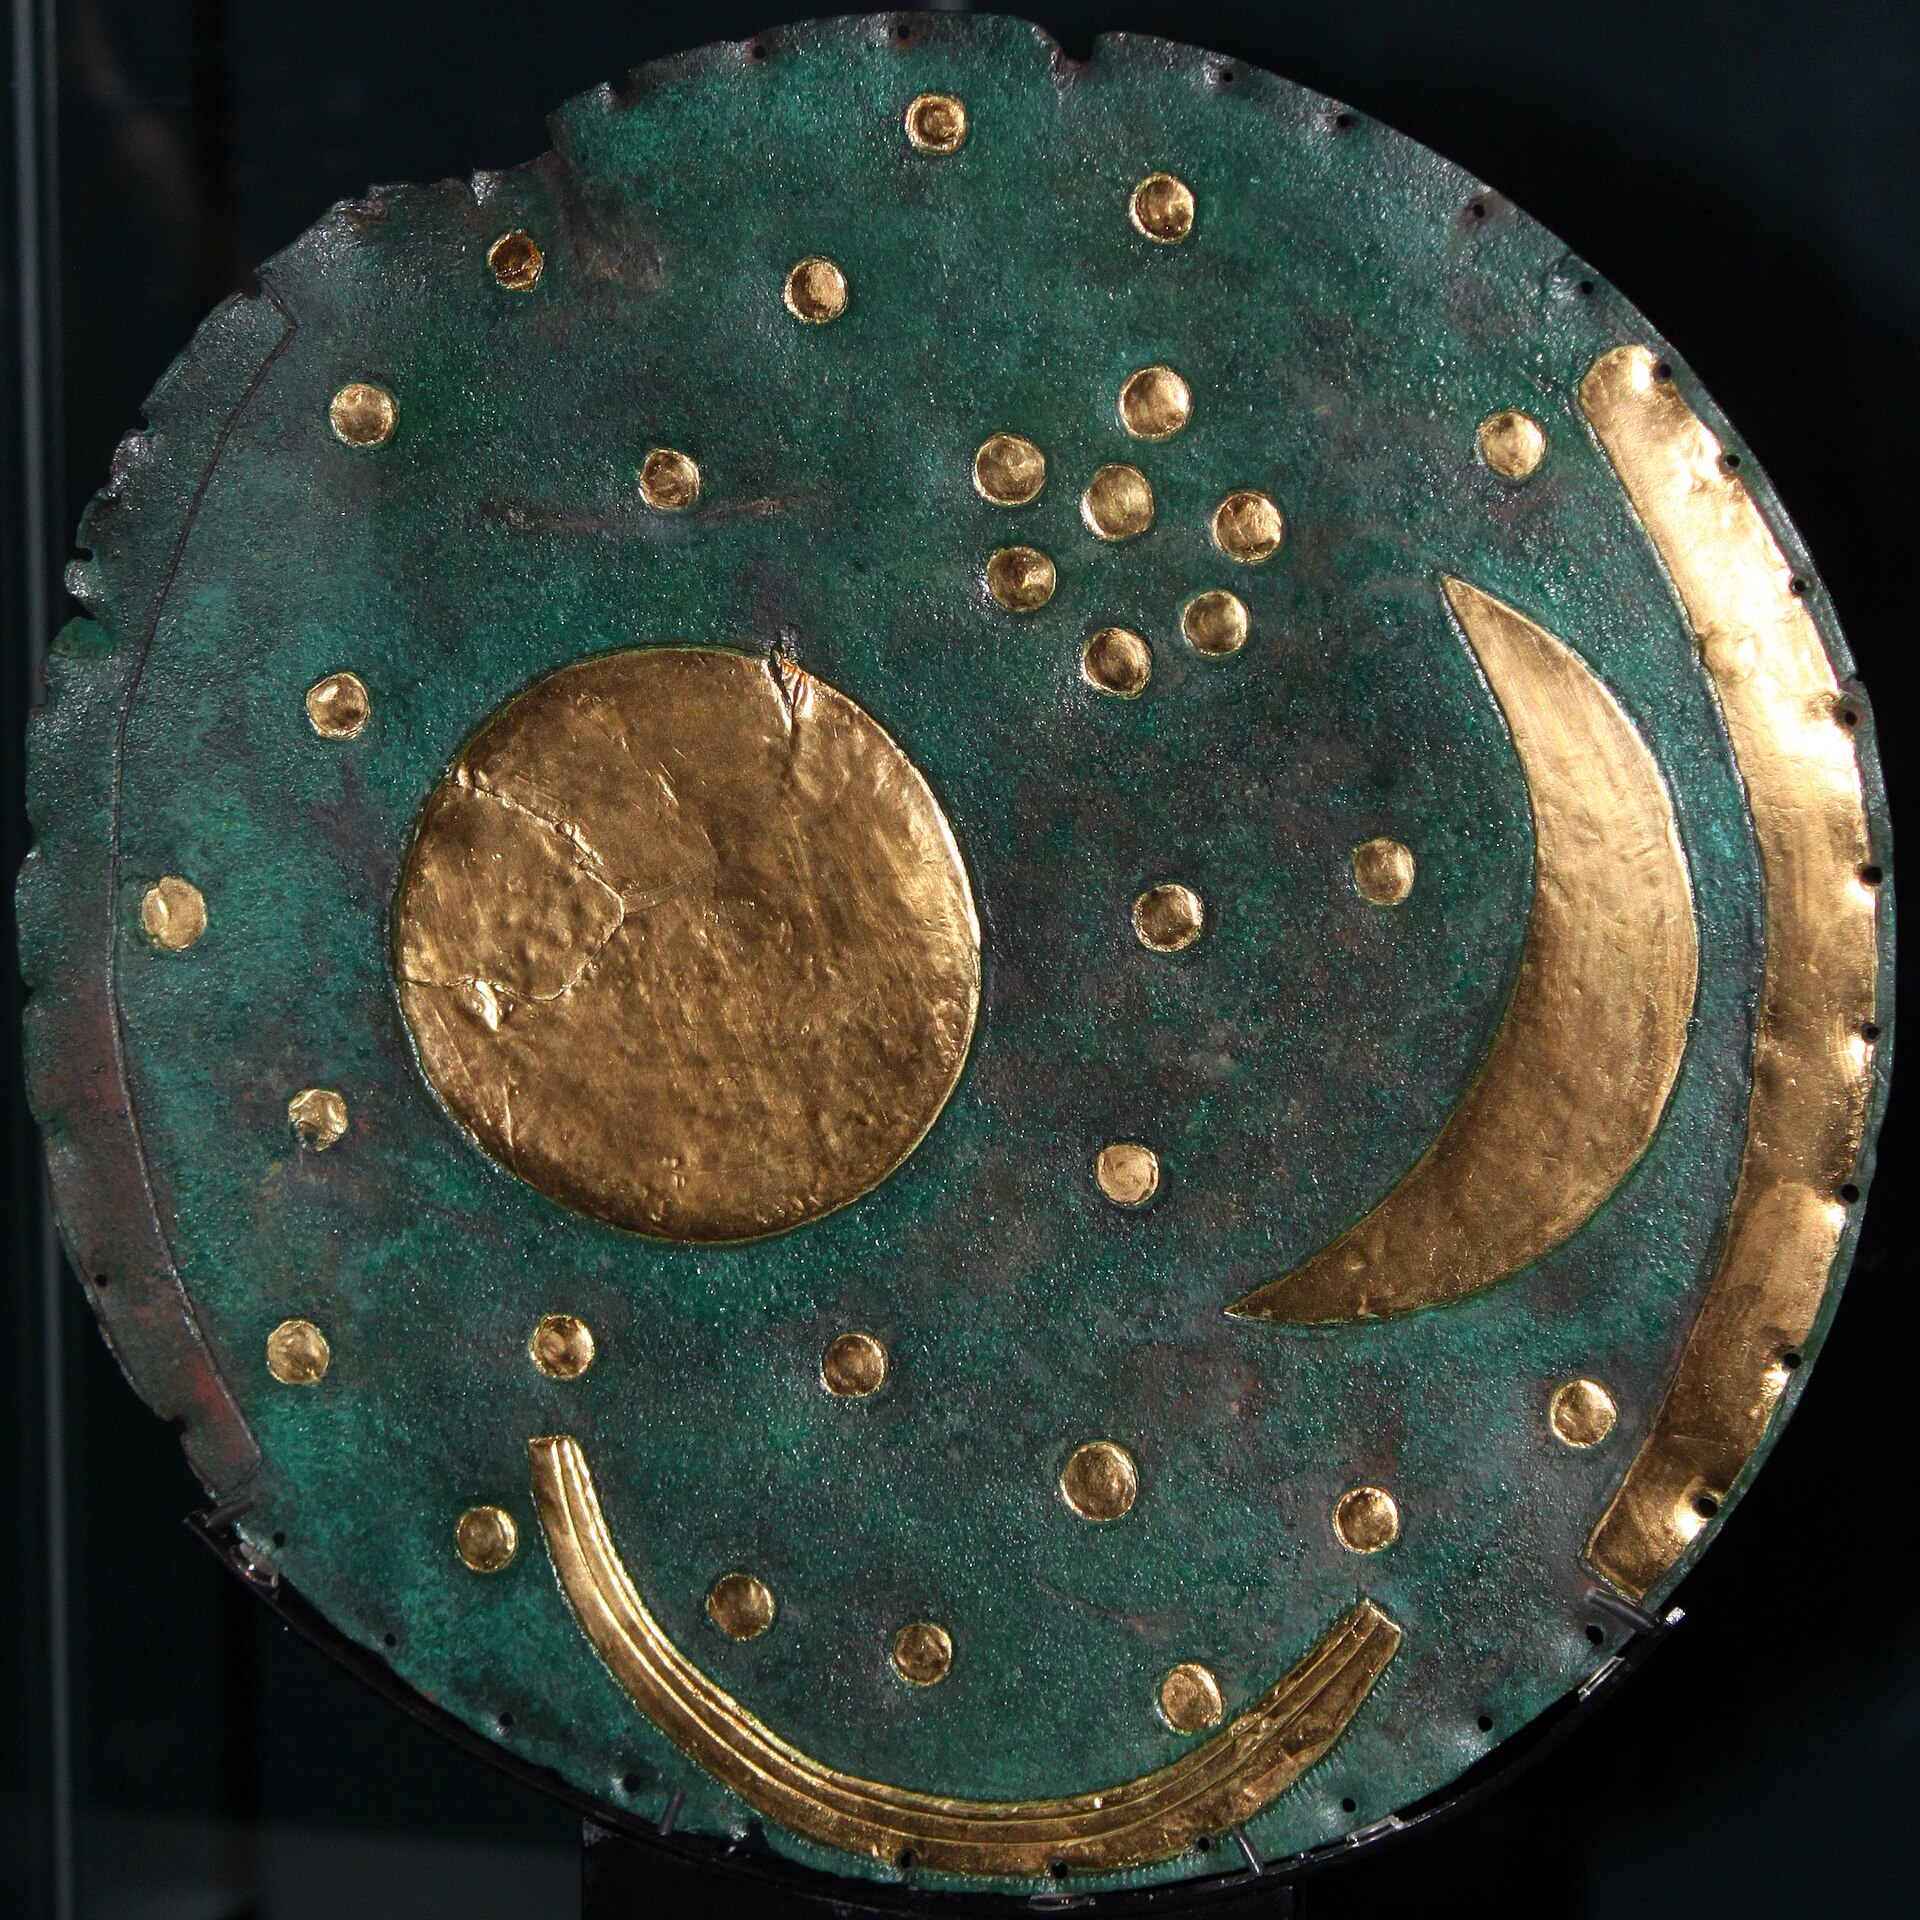
\includegraphics[width=0.52\textwidth]{hist_nebra.jpg}
\caption{The Nebra sky disc, Bronze Age central Germany, usually dated to
around 1600 BCE. Among the gold inlays is a tight cluster of seven dots, set
apart from the scattered single stars, which is widely interpreted as the
Pleiades; the disc is often described as the oldest known concrete depiction of
the night sky. Photograph by Anagoria, public domain, via Wikimedia Commons. \url{https://en.wikipedia.org/wiki/Nebra_sky_disc}}
\end{figure}

Humans had been observing
the Pleiades for thousands of years before written astronomy began. Some of the
earliest surviving evidence comes from ancient Mesopotamia, where the cluster
was known as MUL.MUL, essentially the Stars. Babylonian astronomical
records gave the Pleiades an important position in the organization of the sky
and calendar, and surviving tablets identify the Pleiades with the Babylonian
month Ajaru. The cluster also appears in Mesopotamian astronomical imagery and sources dating to antiquity \cite{bm-k8538,bm-ajaru}.

\begin{figure}[htbp]
\centering
\begin{minipage}[b]{0.40\textwidth}
  \centering
  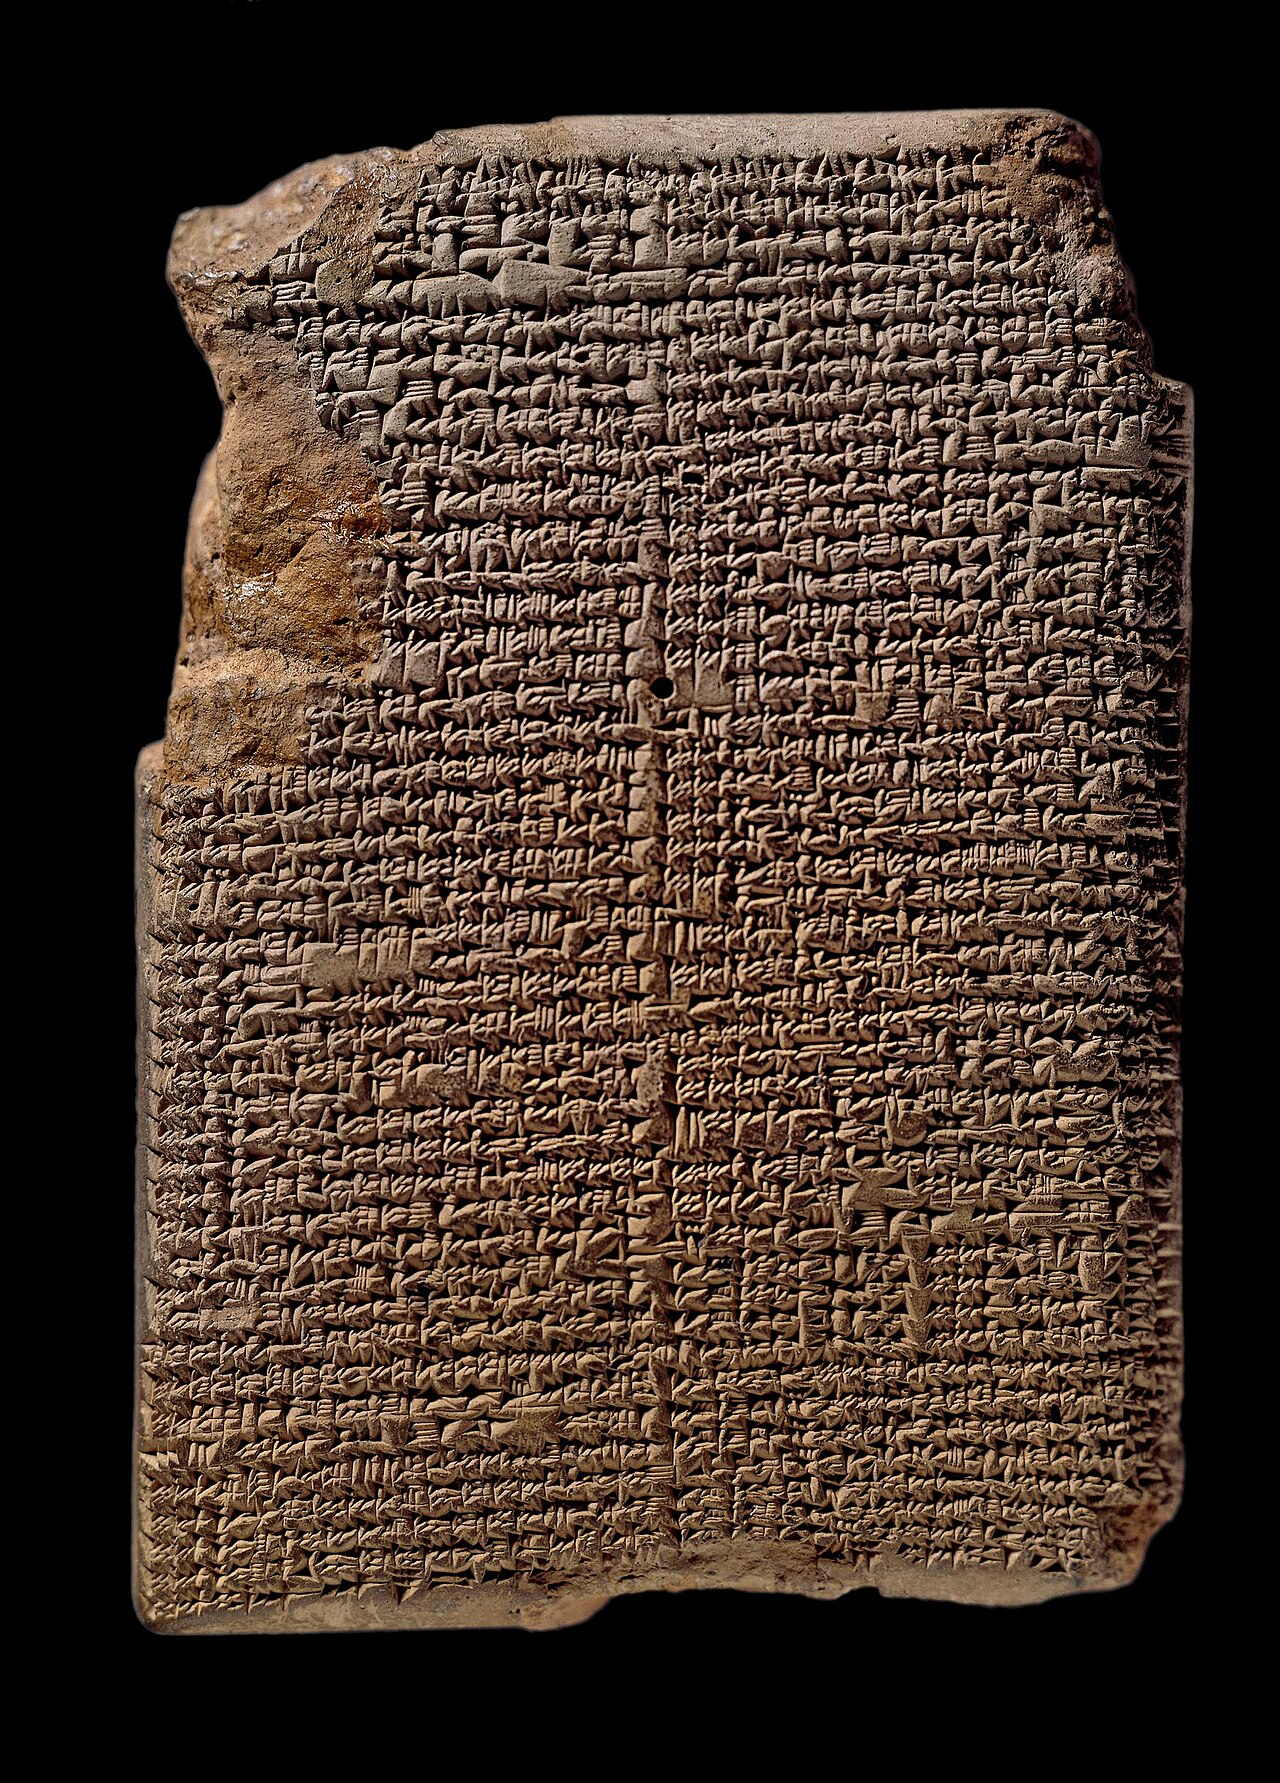
\includegraphics[height=7.2cm]{hist_mulapin.jpg}\\[0.3em]
  {\footnotesize (a) MUL.APIN}
\end{minipage}\hspace{0.04\textwidth}
\begin{minipage}[b]{0.40\textwidth}
  \centering
  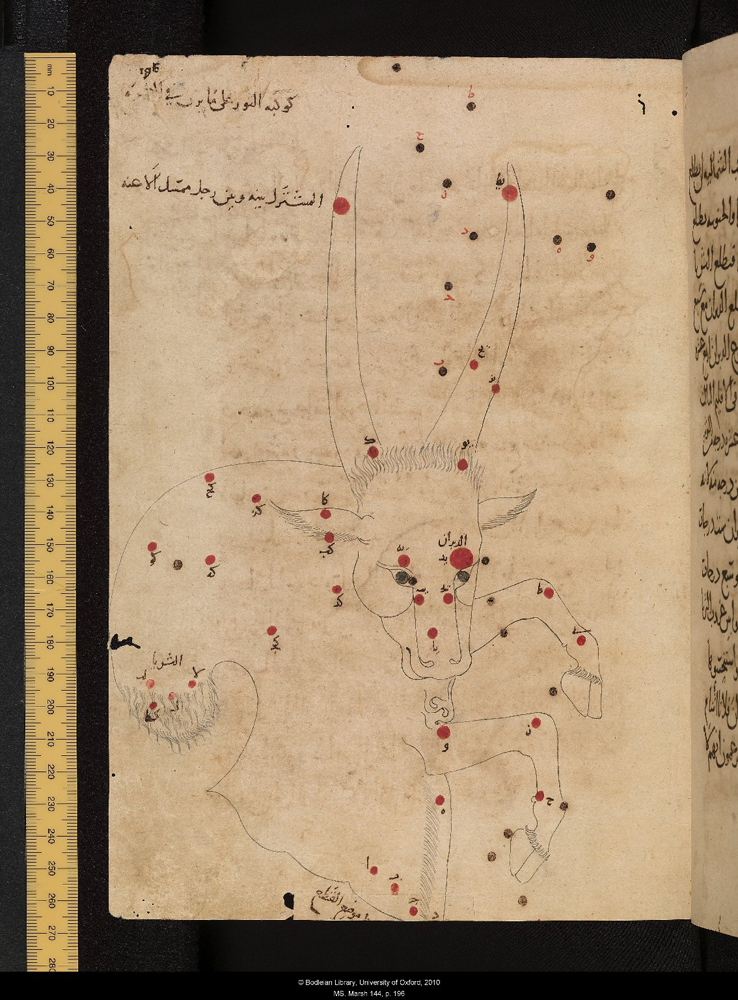
\includegraphics[height=7.2cm]{hist_sufi.jpg}\\[0.3em]
  {\footnotesize (b) Taurus in the \emph{Book of Fixed Stars}}
\end{minipage}
\caption{Two written traditions that recorded the star cluster. (a) MUL.APIN, the
Babylonian compendium of astronomical knowledge, whose catalogue of the stars
in the path of Enlil opens with MUL.MUL, the Pleiades. Image
\copyright~The Trustees of the British Museum, CC BY-SA 4.0, via Wikimedia
Commons. \url{https://en.wikipedia.org/wiki/MUL.APIN\#/media/File:MulApin-BritishMuseum.jpg} 
(b) Taurus as drawn in a copy of al-\d{S}\=uf\={\i}'s
\emph{Book of Fixed Stars} (composed 964 CE; this copy 1009--1010), with the
tight group that Arabic astronomy called al-Thurayy\=a marked among the stars
of the bull. Bodleian Libraries, University of Oxford, MS. Marsh 144, p. 198,
CC BY 4.0. \url{https://commons.wikimedia.org/wiki/File:Book_of_the_Fixed_Stars_Auv0204_taurus.jpg}}
\end{figure}

The cluster also appears very early in Iranian tradition. The Pleiades are
among the few stellar groups named in ancient Iranian sources, eventually
becoming known in Persian as Parvin. Encyclopaedia Iranica notes
that the Pleiades appear in the Younger Avesta (religious book of zoroastrians) which shows the importance
of this particular group of stars in Iranian
tradition at an early period \cite{iranica-constellations}.

Similarly, in ancient Greece, the Pleiades became particularly important practically
and mythologically. The poet Hesiod, writing around the eighth or seventh
century BCE, used their annual movement through the sky as an agricultural
calendar. In Works and Days, he instructed farmers to begin harvesting
when the Pleiades rose and to begin plowing when they set. Their disappearance
and reappearance therefore helped
with structuring the agricultural year \cite{hesiod-works}.

At the same time, Pleiades is denoted as the Seven Sisters in greek mythology, a reference to the
the seven daughters of Atlas and Pleione: Maia, Electra, Taygete, Alcyone,
Celaeno, Sterope or Asterope, and Merope. The association became so deeply embedded 
in cultural tradition that the cluster remains known as the Seven Sisters to this day. \cite{met-pleiades}.
Yet this tradition contains a very interesting underlying problem. Although the mythology
describes seven sisters, most modern observers looking at the cluster with the
naked eye readily distinguish only about six prominent points of light. Ancient
storytellers themselves appear to have been aware of a discrepancy between the
traditional seven and the number that they were seeing. Different Greek (and other ethnicities) traditions
therefore developed explanations for a faint or missing sister. For
example, Merope was sometimes said to have hidden herself or become dim because
she alone among the sisters married a mortal.


Interestingly, traditions involving a group of seven women or sisters
associated with the Pleiades occur far beyond the ancient Mediterranean world.
Among a number of Aboriginal Australian cultures, the Pleiades are associated
with an extensive Seven Sisters tradition. Different communities preserve
different versions. There is, however, a recurring theme that involves a group of ancestral sisters
traveling across the land while being pursued by a male figure. In several
traditions, the sisters eventually escape into the sky and become the Pleiades.
These stories are preserved in songlines extending across enormous areas of
central and western Australia. The National Museum of Australia describes the
Seven Sisters story as occurring across Aboriginal Australia and documents
versions maintained by communities separated by very large geographic distances
\cite{nma-sevensisters,nma-songlines}.

%Other civilizations also independently recognized and named the same
%distinctive cluster, although they did not all literally call it Seven
%Sisters. What remains curious is the fact that geographically separated
%populations repeatedly singled out the Pleiades and often represented them as a
%small collective of related beings. Different traditions include the Japanese
%Subaru, the Indian K\d{r}ttik\={a}, the Persian Parvin, and numerous
%Indigenous interpretations. The Pleiades thus became one of the most culturally
%persistent stellar objects in human history.

What makes the Seven Sisters tradition especially fascinating, however, is that
the sky itself has not remained perfectly unchanged during human history. Stars
are not fixed points attached permanently to a celestial sphere. They are
moving through three-dimensional space, and over sufficiently long periods
their apparent positions relative to one another change. 

This raises an extraordinary possibility concerning the discrepancy between the
traditional seven stars and the roughly six prominent stars that many people see
today.

Two of the important stars in the Pleiades are Atlas and Pleione. Today Pleione
lies so close to the much brighter Atlas from our perspective on Earth that
their light can blend together to the unaided eye. What may appear to us as a
single bright point can therefore contain the light of two distinct stars.
Astronomers Ray Norris and Barnaby Norris examined the measured motions of the
Pleiades and mathematically reconstructed what the cluster may have looked like
in the distant past. Their analysis suggests that roughly 100,000 years ago,
Pleione would have appeared farther from Atlas in the sky than it does today,
potentially making the two much easier for ordinary human vision to
distinguish. In their reconstruction, ancient observers may therefore have been
considerably more likely to perceive seven prominent stars where many observers
today perceive six \cite{norris2021}.

\begin{figure}[htbp]
\centering
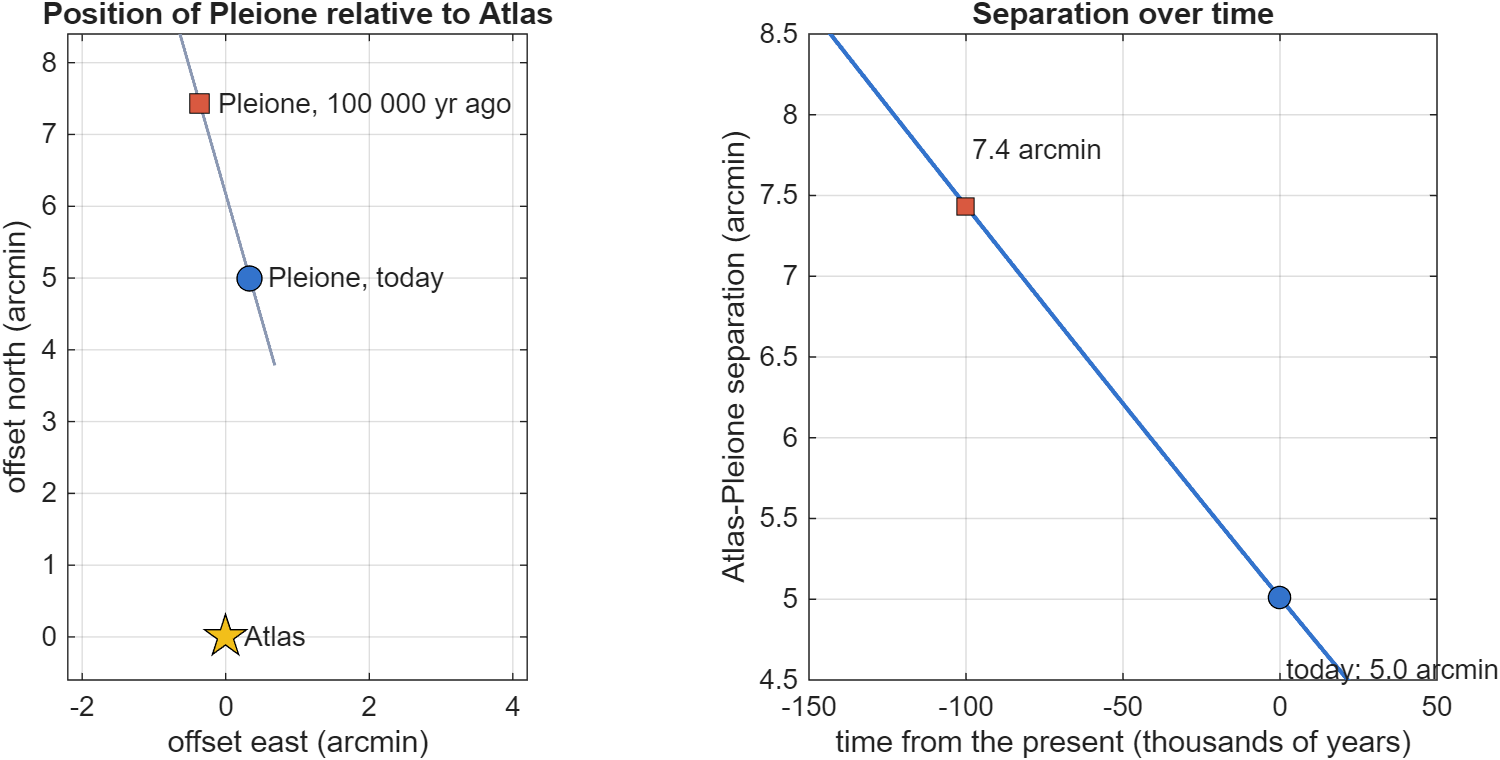
\includegraphics[width=\textwidth]{pleiades_atlas_pleione.png}
\caption{The mechanism, computed from catalogue data. Taking the J2000
positions and proper motions of Atlas (27 Tau) and Pleione (28 Tau) from the
SIMBAD database and extrapolating the relative motion linearly, Pleione stood
about $7.4'$ from Atlas some 100\,000 years ago against about $5.0'$ today, a
separation roughly half as large again. The direction and rough size of the
effect are those described by Norris and Norris \cite{norris2021}. The
extrapolation is deliberately simple: it assumes the present relative velocity
has been constant, ignoring the internal dynamics of the cluster, and
separability by eye depends on the brightness contrast between the two stars
(V = 3.6 against V = 5.1) as well as on the angle.}
\end{figure}

If this reconstruction reflects what prehistoric observers actually saw, it
produces a very interesting scenario. Imagine groups of early humans repeatedly
looking toward this small and distinctive cluster tens of thousands of years
ago. Seven points of light are visible, and stories, names and meanings
gradually become associated with them. Those stories are passed orally from
parents to children and from one generation to another. Human populations
migrate and separate, eventually occupying widely distant regions of the world.
Meanwhile, the stars themselves continue their almost imperceptibly slow motion.

Over thousands of generations, Pleione gradually appears closer to Atlas.
Eventually, the two become sufficiently close from Earth's perspective that most
observers can no longer easily distinguish them as separate naked eye stars. The
sky now seems to contain six prominent points but the inherited story still
says seven. Stories could then provide explanations for what the eye could no longer clearly
see. A sister might have hidden herself, become faint, been separated from the
others, been captured, or disappeared. 


Norris and Norris therefore proposed an extraordinary hypothesis. Perhaps
elements of the Seven Sisters story originated before some of the major
migrations of modern humans out of Africa and were subsequently carried by human
populations as they dispersed across the world. If so, aspects of the story
could conceivably be tens of thousands of years old, perhaps approaching 100,000
years. Under this interpretation, the combination of stellar motion and oral
tradition might explain two mysteries simultaneously: why widely separated
cultures preserve surprisingly similar stories surrounding the Pleiades, and why
traditions repeatedly emphasize seven figures even though many modern observers
see only six \cite{norris2021}.



The Seven Sisters therefore represent one of humanity's
oldest continuous relationships with the natural world and tell a story transmitted
across generations.

The Pleiades problem of the Bari test set follows
seven bodies of masses $m_i = i$ moving in a plane under mutual gravitation ---
seven points of light whose motion, here, is computed rather than remembered.

\section{Problem statement}

\begin{quote}

\medskip
1. (100 points) Consider the Pleiades problem of the University of Bari ODE
Benchmark ODE Benchmark provided as equations (II.6.3) in page II-6-1 of the
document, or equivalently,

\begin{enumerate}
\renewcommand{\labelenumi}{(\alph{enumi})}

\item Write in a MATLAB Pleiades.m file the code for the right-hand-side of the
E5 model.

\item Solve Pleiades using relative tolerances (rtol), absolute tolerances
(atol), and initial step size $h_0$ given respectively by
\[
\begin{array}{lll}
\text{rtol} = 10^{-4},  & \text{atol} = \text{rtol}\,, & h_0 = 10^{-6}\\[0.2em]
\text{rtol} = 10^{-7},  & \text{atol} = \text{rtol}\,, & h_0 = 10^{-9}\\[0.2em]
\text{rtol} = 10^{-10}, & \text{atol} = \text{rtol}\,, & h_0 = 10^{-12}
\end{array}
\]
using MATLAB ODE solvers ode45, ode23, ode113, ode15s, ode23s, ode23t, ode23tb,
where the first three are non-stiff ODE solvers and the last four are stiff ODE
solvers.

\item Make a plot, as in Figure II.6.2, of the evolution of $x_1, y_1$, using one
of the solvers you used with one of the triple $(\text{rtol}, \text{atol}, h_0)$
given in the previous item.

\item For each run report in a table (like Table II.6.2) with columns solver
name, rtol (relative tolerance), atol (absolute tolerance), $h_0$ (initial time
step), mescd (the minimum number of mixed significant correct digits in the
numerical solution at the end of the integration interval)
\[
\text{mescd} = -\log_{10}
\left( \left\lVert y_{\text{approximated}} - y_{\text{true}} \right\rVert_{\infty}
\Big/ \left( \frac{\text{atol}}{\text{rtol}}
+ \left\lVert y_{\text{true}} \right\rVert_{\infty} \right) \right),
\]
where
\[
\lVert (w_1, \cdots, w_n)^{T} \rVert_{\infty} = \max_{1 \leq i \leq n} \{ |w_i| \},
\]
scd (the minimum number of significant correct digits in the numerical solution
at the end of the integration interval)
{\footnotesize
\[
\text{scd} =
\begin{cases}
-\log_{10}\left( \lVert (y_{\text{approximated}} - y_{\text{true}})
 ./ (y_{\text{true}}) \rVert_{\infty} \right), &
\text{if } |y_{true,i}| \geq 10^{-12},\ i = 1, \cdots, n\\[0.9em]
-\log_{10}\left( \lVert y_{\text{approximated}} - y_{\text{true}}
 \rVert_{\infty} \right), &
\text{if } |y_{\text{true},i}| < 10^{-12}, \text{for some } i \in \{1, \cdots, n\},
\end{cases}
\]
}
steps (number of steps), accept (number of accepted steps), \#f (number of
function evaluations), \#Jac (number of Jacobian evaluations), \#LU (number of
LU systems solved) and CPU (CPU time, measured as the minimum time of running
the ODE solver five times).

\item Comment on your results utilizing the table generated. Do not forget to
provide the table.

\item As deliverables, you will need to provide (via email) your source code for
all the simulations, the generation of the graphic, the generation of the table,
with instructions about how to run your code in interactive mode, and a text
file Pleiades.txt with your comments about the table columns.
\end{enumerate}

\medskip
Pleiades derivation: For any body $i$, the net gravitational force exerted on it
by all other bodies $j \neq i$ is the vector sum of individual attractive
forces:
\[
F_i = \sum_{j \neq i} \frac{G m_i m_j}{|r_j - r_i|^{3}} \left( r_j - r_i \right)
\]
By substituting $G = 1$ and applying Newton's second law
($F_i = m_i r_i^{''}$), the mass $m_i$ cancels out, leaving the acceleration
vector
\[
r_i^{''} = \sum_{j \neq i} \frac{m_j}{|r_j - r_i|^{3}} \left( r_j - r_i \right)
\]
\end{quote}


\section{The problem}

Seven bodies of masses $m_i = i$, $i = 1,\dots,7$, move in a plane under mutual
gravitation with the gravitational constant set to one. Newton's second law and
the law of gravity gives, after the mass $m_i$ cancels,
\begin{equation}
\ddot{x}_i = \sum_{j \neq i} \frac{m_j (x_j - x_i)}{r_{ij}^{3/2}},
\qquad
\ddot{y}_i = \sum_{j \neq i} \frac{m_j (y_j - y_i)}{r_{ij}^{3/2}},
\qquad
r_{ij} = (x_i - x_j)^2 + (y_i - y_j)^2 ,
\label{eq:accel}
\end{equation}
which is (II.6.2). Note that $r_{ij}$ is the squared distance meaning the
exponent is $3/2$ instead of $3$. We can then write $z = (x^{T}, y^{T})^{T} \in
\mathbb{R}^{14}$ and $w = z'$ turns this into the first order system (II.6.3)
\begin{equation}
z' = w, \qquad w' = f(z),
\label{eq:first-order}
\end{equation}
of dimension 28, integrated over $0 \le t \le 3$ from
\begin{align*}
x(0)  &= (3,\,3,\,-1,\,-3,\,2,\,-2,\,2)^{T}, &  y(0)  &= (3,\,-3,\,2,\,0,\,0,\,-4,\,4)^{T},\\
x'(0) &= (0,\,0,\,0,\,0,\,0,\,1.75,\,-1.5)^{T}, & y'(0) &= (0,\,0,\,0,\,-1.25,\,1,\,0,\,0)^{T}.
\end{align*}

The problem is non-stiff, and during the motion several quasi-collisions
occur (Table II.6.1): the closest is between bodies 1 and 7 at $t \approx 1.68$,
where the squared distance falls to $0.0011$. Since the right-hand side
\eqref{eq:accel} behaves like $r_{ij}^{-3/2}$, these near misses are where the
solution changes character abruptly, where the step size controller is forced
down, and where local errors are amplified. They govern everything in the table
of Section~\ref{sec:table}.

\section{Part a: the right-hand side}

We can take the $28$ differential equations corresponding to the seven stars and their 
$x$ and $y$ positions as well as their respective horizontal and vertical velocities and put them all in one vector:
\[
u = \bigl[\,x_1..x_7,\; y_1..y_7,\; x'_1..x'_7,\; y'_1..y'_7\,\bigr]^{T} \in \mathbb{R}^{28},
\]
therefore $u_1 = x_1$ and $u_8 = y_1$. In the \texttt{Pleiades.m} script, we implement
Equation~\ref{eq:first-order} using matrix operations.
We first calculate the pairwise differences between
the stars' coordinates and store them in matrices.
We then set the diagonal entries of the distance
matrix to infinity to exclude self-interactions
($j=i$). Finally, we calculate the accelerations
in both directions using matrix-vector multiplication
with the mass vector:

\begin{quote}
\begin{verbatim}
m = (1:7)';                     %masses mi = i
x  = u(1:7);
y  = u(8:14);

DX = x.' - x;                   %DX(i,j) = xj - xi
DY = y.' - y;

R32 = (DX.^2 + DY.^2).^(3/2);   %rij is the SQUARED distance
R32(1:8:end) = Inf;             %drop the i = j terms

ax = (DX ./ R32) * m;
ay = (DY ./ R32) * m;

du = [u(15:28); ax; ay];
\end{verbatim}
\end{quote}

If we integrate using \code{ode113} at tolerance
$\text{rtol} = \text{atol} = 10^{-13}$ we would be able to reproduce the reference solution of
Table II.6.2 at $t = 3$ to a maximum absolute error of
$2.9 \times 10^{-11}$ in the 14 positions and $6.0 \times 10^{-11}$ in the 14
velocities, which confirms both the formula and the ordering of the state vector.

\section{Part b: numerical performance and tolerance sensitivity analysis}

Using the script \code{run\_pleiades.m} we ran seven solvers over the three triples, $21$
configurations in all. We set tolerances with \code{odeset('RelTol',\dots,
'AbsTol',\dots)} and the initial step with the \code{'InitialStep'} script. We then ran each
configuration three separate ways for three different purposes:

\begin{enumerate}
\item once with \code{'Stats','on'} in order to capture the printed counters with
      \code{evalc} and parse them (\code{pleiades\_\allowbreak parsestats.m}) to obtain
      the accepted and failed steps, the Jacobian evaluations, the LU
      decompositions and the linear solves, as well as the end-point solution
      used for the accuracy measures;
\item once through a counting wrapper around the right-hand side, which gave us an
      exact count of function evaluations. MATLAB prints large counters in
      \code{\%g} format and therefore loses digits above $10^5$;
\item five more times with statistics off and the plain right-hand side, taking
      the minimum wall-clock time as the CPU column, as part d requires.
\end{enumerate}

One issue encountered during the timing tests was that calling a MATLAB
ODE solver without output arguments automatically invokes \texttt{odeplot},
which plots the solution during integration and significantly increases
execution time. An earlier version of the timing loop unintentionally
included this overhead and reported 60.8~s for \texttt{ode23s} at
$\mathrm{rtol}=10^{-10}$ instead of the actual 11.0~s. This resulted in
execution times being overestimated by approximately a factor of six.
To avoid this issue, all solver calls in the final code explicitly
request output arguments.

The end-point solution of every run is stored in \code{pleiades\_results.mat} as a
$21 \times 28$ matrix. Therefore, the accuracy measures can be recomputed under a
different convention without repeating any integration.

\section{Part c: evolution of $x_1$ and $y_1$}

\begin{figure*}[ht]
\centering
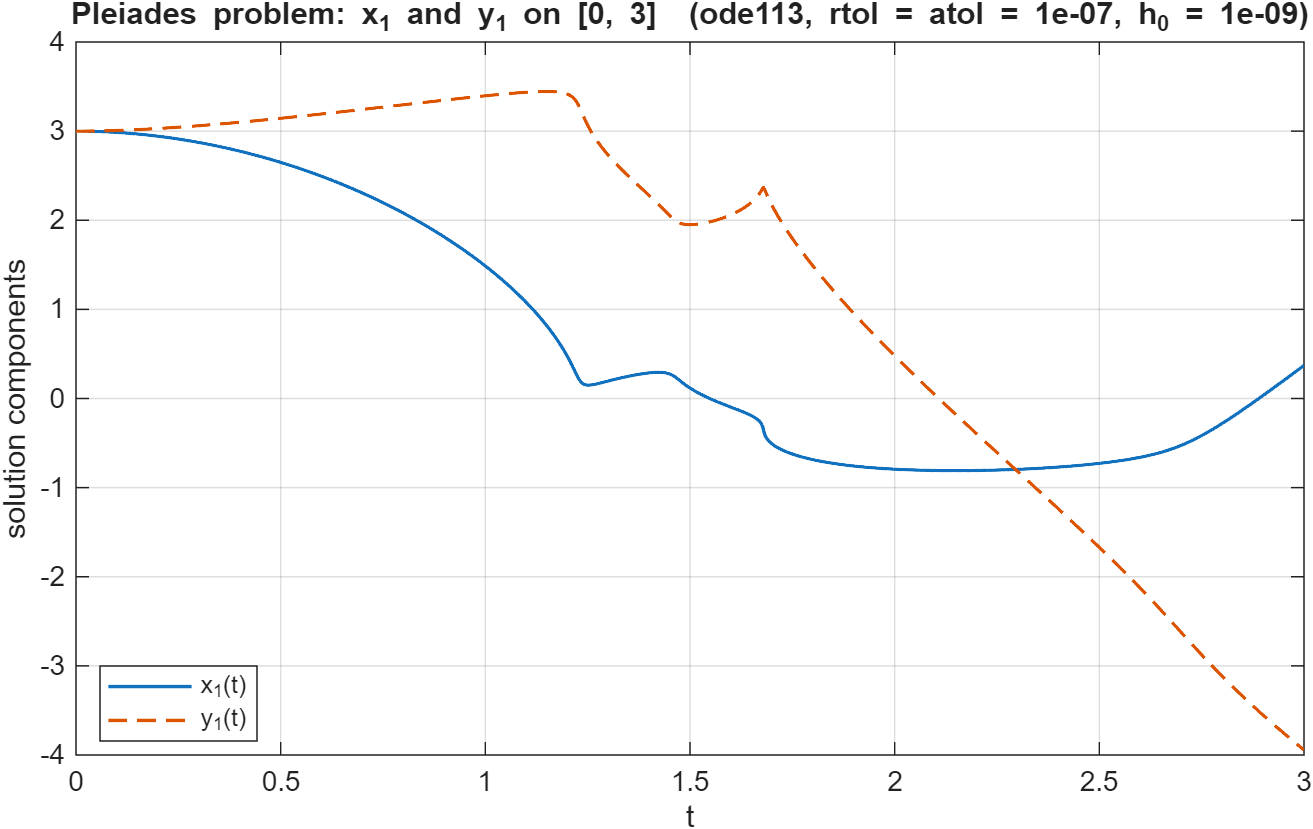
\includegraphics[width=0.92\textwidth]{pleiades_x1y1.png}
\caption{Solution components $x_1$ and $y_1$ over $[0,3]$, computed with
\code{ode113} at $\text{rtol} = \text{atol} = 10^{-7}$, $h_0 = 10^{-9}$
(\code{pleiades\_figure.m}). The kinks at $t \approx 1.23$, $1.46$ and $1.68$ are
the three quasi-collisions of Table II.6.1 that involve body 1. The end values
$x_1(3) = 0.3706$ and $y_1(3) = -3.943$ agree with Table II.6.2.}
\end{figure*}

\section{Part d: the table of run characteristics}
\label{sec:table}

\subsection*{The two accuracy measures}

Both are evaluated at $t = 3$ against the reference solution of Table II.6.2,
using the definitions given in the assignment:
\begin{equation}
\text{mescd} = -\log_{10}
\left( \frac{\lVert u - u_{\text{ref}} \rVert_{\infty}}
            {\frac{\text{atol}}{\text{rtol}} + \lVert u_{\text{ref}} \rVert_{\infty}} \right),
\qquad
\text{scd} = -\log_{10}
\left\lVert \frac{u - u_{\text{ref}}}{u_{\text{ref}}} \right\rVert_{\infty},
\label{eq:measures}
\end{equation}
where $\lVert \cdot \rVert_{\infty}$ is the largest absolute value over the
components and the division in scd is element by element. (The second form of
scd, $-\log_{10}\lVert u - u_{\text{ref}}\rVert_{\infty}$, applies when some
$\lvert u_{\text{ref},i} \rvert < 10^{-12}$. Since all reference components 
are of order one, the relative form is used.)

Two details are important when interpreting the accuracy measures.

First, mescd is not calculated separately for each component.
Instead, both norms are taken over the entire vector and the largest
absolute error is scaled by a single value:

\[
\frac{\mathrm{atol}}{\mathrm{rtol}}
+\lVert u_{\mathrm{ref}}\rVert_{\infty}
=1+5.2251=6.2251.
\]

For these runs, mescd therefore measures the largest absolute error
in terms of decimal digits, with an additional constant of
$\log_{10}(6.2251)=0.794$. This definition is useful when a solution
component approaches zero, since relative errors can become very
large even when the absolute error remains small.

Second, mescd and scd use different sets of components, following
the conventions of the reference test set. For mescd, all 28
components are included, as the test set specifies that
all the components of the solution are taken into account
(page II-ii). For scd, only the first 14 components, corresponding
to the positions, are used, as specified for the Pleiades problem
(page II-6-3). These component sets are defined by
\texttt{P.imescd} and \texttt{P.iscd} in
\texttt{pleiades\_setup.m}.

Using only the 14 position components for mescd would increase
the reported values by approximately 0.1 to 0.6 digits. For
example, the mescd value for \texttt{ode45} at
$\mathrm{rtol}=10^{-4}$ would increase from 2.11 to 2.37.
This happens because the largest absolute errors generally
occur in the velocity components.

It is also important to note that the original test set uses a
different definition of mescd (formula II.2, page II-ii),
which calculates the error component by component:

\[
-\log_{10}\left\lVert
e \mathbin{./}
\left(\mathrm{atol}+\mathrm{rtol}\cdot u_{\mathrm{ref}}\right)
\right\rVert_{\infty}.
\]

As a result, the mescd values reported in Table II.6.3 cannot
be directly compared with those obtained in this study.
However, since the definitions of scd are the same in both cases, 
those results can be compared, as discussed in
Section~\ref{sec:discussion}.


We note that in part d, the column labeled ``\#LU (number of LU systems solved)''
may be somewhat ambiguous, as it could refer to either LU factorizations
or the linear systems solved using those factorizations. MATLAB reports
these quantities separately, while the reference test set reports
the number of LU decompositions (page II-ii). For clarity, we included both
quantities in our results. This distinction is important
for understanding the efficiency of implicit solvers. For a dense
system of size $n$, an LU factorization requires $O(n^3)$ operations,
whereas solving a system using an existing factorization requires
only $O(n^2)$ operations. By reusing factorizations for multiple
solves, implicit methods can significantly reduce their computational
cost.

\subsection*{The table}

\begin{center}
\footnotesize
\setlength{\tabcolsep}{3.5pt}
\begin{tabular}{lcccrrrrrrrrr}
\toprule
solver & rtol & atol & $h_0$ & mescd & scd & steps & accept & \#f & \#Jac & \#LU & \#solve & CPU \\
\midrule
\texttt{ode45} & $10^{-4}$ & $10^{-4}$ & $10^{-6}$ & 2.11 & 1.14 & 127 & 106 & 763 & -- & -- & -- & 0.0057 \\
\texttt{ode45} & $10^{-7}$ & $10^{-7}$ & $10^{-9}$ & 5.70 & 4.77 & 371 & 371 & 2\,227 & -- & -- & -- & 0.0139 \\
\texttt{ode45} & $10^{-10}$ & $10^{-10}$ & $10^{-12}$ & 9.51 & 8.84 & 1\,465 & 1\,465 & 8\,791 & -- & -- & -- & 0.0523 \\
\addlinespace
\texttt{ode23} & $10^{-4}$ & $10^{-4}$ & $10^{-6}$ & 2.47 & 1.82 & 464 & 460 & 1\,393 & -- & -- & -- & 0.0089 \\
\texttt{ode23} & $10^{-7}$ & $10^{-7}$ & $10^{-9}$ & 5.54 & 4.84 & 4\,584 & 4\,584 & 13\,753 & -- & -- & -- & 0.0808 \\
\texttt{ode23} & $10^{-10}$ & $10^{-10}$ & $10^{-12}$ & 8.54 & 7.84 & 45\,793 & 45\,793 & 137\,380 & -- & -- & -- & 0.8093 \\
\addlinespace
\texttt{ode113} & $10^{-4}$ & $10^{-4}$ & $10^{-6}$ & 2.07 & 1.48 & 363 & 343 & 707 & -- & -- & -- & 0.0056 \\
\texttt{ode113} & $10^{-7}$ & $10^{-7}$ & $10^{-9}$ & 5.31 & 4.33 & 679 & 657 & 1\,337 & -- & -- & -- & 0.0104 \\
\texttt{ode113} & $10^{-10}$ & $10^{-10}$ & $10^{-12}$ & 8.36 & 7.71 & 1\,128 & 1\,110 & 2\,239 & -- & -- & -- & 0.0172 \\
\addlinespace
\texttt{ode15s} & $10^{-4}$ & $10^{-4}$ & $10^{-6}$ & 1.40 & 0.74 & 522 & 463 & 795 & 1 & 112 & 766 & 0.0087 \\
\texttt{ode15s} & $10^{-7}$ & $10^{-7}$ & $10^{-9}$ & 4.27 & 3.59 & 1\,397 & 1\,327 & 1\,612 & 1 & 178 & 1\,581 & 0.0219 \\
\texttt{ode15s} & $10^{-10}$ & $10^{-10}$ & $10^{-12}$ & 6.70 & 6.04 & 4\,125 & 4\,048 & 4\,610 & 1 & 351 & 4\,579 & 0.0509 \\
\addlinespace
\texttt{ode23s} & $10^{-4}$ & $10^{-4}$ & $10^{-6}$ & 1.98 & 1.01 & 592 & 590 & 18\,295 & 590 & 592 & 1\,776 & 0.1112 \\
\texttt{ode23s} & $10^{-7}$ & $10^{-7}$ & $10^{-9}$ & 4.14 & 3.21 & 5\,875 & 5\,875 & 182\,138 & 5\,875 & 5\,875 & 17\,625 & 1.1018 \\
\texttt{ode23s} & $10^{-10}$ & $10^{-10}$ & $10^{-12}$ & 6.16 & 5.23 & 58\,702 & 58\,702 & 1\,819\,765 & 58\,702 & 58\,702 & 176\,106 & 11.2093 \\
\addlinespace
\texttt{ode23t} & $10^{-4}$ & $10^{-4}$ & $10^{-6}$ & 1.49 & 0.61 & 808 & 807 & 1\,340 & 1 & 136 & 1\,311 & 0.0113 \\
\texttt{ode23t} & $10^{-7}$ & $10^{-7}$ & $10^{-9}$ & 3.51 & 2.67 & 8\,160 & 8\,160 & 8\,360 & 1 & 154 & 8\,329 & 0.0668 \\
\texttt{ode23t} & $10^{-10}$ & $10^{-10}$ & $10^{-12}$ & 5.48 & 4.73 & 81\,309 & 81\,309 & 81\,498 & 1 & 159 & 81\,467 & 0.6390 \\
\addlinespace
\texttt{ode23tb} & $10^{-4}$ & $10^{-4}$ & $10^{-6}$ & 1.59 & 0.74 & 643 & 642 & 2\,101 & 1 & 133 & 2\,715 & 0.0171 \\
\texttt{ode23tb} & $10^{-7}$ & $10^{-7}$ & $10^{-9}$ & 3.60 & 2.82 & 6\,419 & 6\,419 & 19\,268 & 1 & 155 & 25\,656 & 0.1422 \\
\texttt{ode23tb} & $10^{-10}$ & $10^{-10}$ & $10^{-12}$ & 5.62 & 4.68 & 64\,257 & 64\,257 & 192\,614 & 1 & 164 & 256\,840 & 1.4192 \\
\bottomrule
\end{tabular}

\end{center}

\footnotesize
steps $=$ accepted $+$ failed attempts. CPU in seconds, minimum of five runs,
MATLAB R2025a on Windows 11. A dash marks a counter the solver does not report:
\code{ode45}, \code{ode23} and \code{ode113} are explicit and form neither
Jacobians nor linear systems.
\normalsize

\section{Part e: discussion}
\label{sec:discussion}

The three non-stiff solvers consistently outperform the stiff solvers
at all three tolerance levels. At $\mathrm{rtol}=10^{-10}$,
\texttt{ode113} achieves 7.71 correct digits in just 0.017~s
with 2,239 function evaluations. In comparison, \texttt{ode23s}
requires 11.2~s and approximately 1.82 million function evaluations,
while achieving only 5.23 correct digits. This makes
\texttt{ode23s} roughly 650 times slower, despite producing about
2.5 fewer correct digits.

We note that this difference does not necessarily mean that the stiff solvers are
less effective. They perform additional computations,
including Jacobian evaluations, matrix factorizations, and Newton
iterations, that provide little benefit for this non-stiff problem.
In the Pleiades system, the step size is primarily determined by
the accuracy required during close encounters between the stars,
instead of numerical stability restrictions. As a result,
solvers designed for non-stiff problems are better suited to
this system and achieve greater accuracy with significantly
less computational effort.

Reducing the tolerance by six orders of magnitude leads to a substantial
increase in the number of steps required by most solvers. The step
counts increase by the following factors:

\[
\begin{array}{ll}
\texttt{ode23}: 98.7\times, &
\texttt{ode23t}: 100.6\times,\\
\texttt{ode23tb}: 99.9\times, &
\texttt{ode23s}: 99.2\times,\\
\texttt{ode45}: 11.5\times, &
\texttt{ode113}: 3.1\times,\\
\texttt{ode15s}: 7.9\times. &
\end{array}
\]

These results are consistent with the classical relationship
$\mathrm{steps}\sim\mathrm{tol}^{-1/(q+1)}$, where $q$ is the order
of the numerical method. For a second-order method ($q=2$),
this relationship predicts a 100-fold increase in the step count,
which closely matches the results for \texttt{ode23},
\texttt{ode23t}, \texttt{ode23tb}, and \texttt{ode23s}.
For \texttt{ode45}, using $q=4$ predicts an increase of
approximately 15.8 times, compared with the observed factor of 11.5.

Among all the solvers, \texttt{ode113} shows the smallest increase
in step count, at only 3.1 times. Its ability to adjust the method
order allows it to maintain efficiency as the tolerance becomes
more restrictive. At $\mathrm{rtol}=10^{-10}$, it is also the
fastest solver in the comparison. Meanwhile, \texttt{ode45}
achieves the highest accuracy, with $\mathrm{scd}=8.84$,
while requiring only 0.052~s of computation time.

At $\mathrm{rtol}=10^{-4}$, none of the solvers achieves two
correct digits, with scd values ranging from 0.61 to 1.82.
This indicates that the numerical errors affect even the
leading digits of the final positions. The three close
encounters involving body 1, shown in the figure in part c,
can amplify errors accumulated during integration and
contribute to the loss of accuracy.

This behavior highlights an important distinction between
local and global error. The specified tolerance controls
the estimated local error at each integration step, but
does not guarantee the same level of accuracy in the
final solution. Because the Pleiades system is sensitive
to accumulated numerical errors, a tolerance of $10^{-4}$
does not necessarily produce four correct digits.
Therefore, the accuracy of each solver should be evaluated
by comparing its results with a reliable reference solution.


From $\text{rtol} = 10^{-4}$ to $10^{-10}$, \code{ode45} improves from
$\text{scd} = 1.14$ to $8.84$, about $1.3$ digits per decade, and \code{ode23}
from $1.82$ to $7.84$. The stiff solvers gain less: \code{ode23t} goes from
$0.61$ to $4.73$, about $0.7$ digits per decade, and stays two to four digits
behind the explicit solvers at equal tolerance.

The mescd values are higher than the scd values in all 21 runs,
with differences ranging from 0.59 to 0.98 digits. Because the two measures in
Equation~\ref{eq:measures} use different components and scaling
methods, this difference is not constant.

The mescd measure considers the largest absolute error across
all 28 components and scales it by a single constant, 6.2251.
In every run, the largest absolute error occurs in a velocity
component, most commonly $x'_5$ or $x'_1$. These components
tend to have relatively large values and change rapidly
throughout the simulation.

In contrast, scd considers only the 14 position components
and divides each error by its corresponding reference value.
The largest relative error occurs in $x_1$, with a reference
value of 0.3706, in most runs, and in $x_5$, with a reference
value of 0.3426, in the remaining runs. These are the two
smallest reference positions in absolute value, making their
relative errors more sensitive to a given absolute error.

As a result, the difference between mescd and scd depends
on how the numerical errors are distributed between the
position and velocity components. Since this distribution
changes across solvers and tolerance levels, the gap between
the two measures also varies. Despite these differences,
both measures give the same ranking of solvers in this
experiment. However, their results could differ substantially
if a reference position were close to zero at $t=3$.


The solvers \texttt{ode15s}, \texttt{ode23t}, and
\texttt{ode23tb} each evaluate the Jacobian only once
during the entire integration, regardless of the tolerance.
They also perform relatively few LU factorizations, ranging
from 112 to 351. This suggests that the Newton iterations
converge efficiently for this non-stiff problem and allow
MATLAB to reuse the same Jacobian without repeatedly
recomputing it. For example, at $\mathrm{rtol}=10^{-10}$,
\texttt{ode23t} performs 81,467 linear solves using only
159 LU factorizations, with 81,498 function evaluations,
approximately one per step.

In contrast, \texttt{ode23s} requires considerably more
computation. Its Rosenbrock method uses the Jacobian directly
in its numerical formula, and the results show that a new
Jacobian and LU factorization are computed at every step.
At $\mathrm{rtol}=10^{-10}$, the solver performs 58,702
Jacobian evaluations, 58,702 LU factorizations, and
176,106 linear solves, corresponding to three solves
per step, one for each stage.

For this 28-dimensional system, approximating each Jacobian
numerically requires approximately 28 additional evaluations
of the right-hand-side function. This accounts for much of
the approximately 1.82 million function evaluations reported
for \texttt{ode23s}. In addition, repeatedly performing LU
factorizations, which require $O(n^3)$ operations for a
dense system of size $n$, adds substantial computational cost.
These factors explain why \texttt{ode23s} is the
slowest solver in the comparison.

Providing an analytical Jacobian could reduce the number
of function evaluations by avoiding the additional evaluations
needed for numerical approximation. However, it would not
eliminate the cost of repeated LU factorizations. Therefore,
\texttt{ode23s} would likely remain less efficient than the
other solvers for this non-stiff problem.

The difference between attempted and accepted steps is largest at
$\mathrm{rtol}=10^{-4}$. At this tolerance, \texttt{ode45}
rejects 21 out of 127 attempted steps, while \texttt{ode15s}
rejects 59 out of 522. As the tolerance becomes more restrictive,
the number of rejected steps decreases, reaching zero for most
solvers at $\mathrm{rtol}=10^{-10}$.

We can explain this behavior through how the solvers adjust their step
sizes. With a larger tolerance, the solvers initially attempt
larger steps, which may produce excessive errors during close
encounters between the stars. These steps are then rejected,
forcing the solvers to reduce their step sizes and try again.
With tighter tolerances, the solvers already take smaller steps which makes
it less likely that the estimated error will exceed the
allowed limit.

The initial step sizes of $10^{-6}$, $10^{-9}$, and $10^{-12}$
are much smaller than necessary at $t=0$, where the solution
is relatively smooth. However, the adaptive solvers adjust
their step sizes within the first few steps such that the small
initial values have little effect on the overall computation.
Although they may introduce a few additional steps, they
also help prevent the solver from starting with a step that
is too large. Therefore, the initial step size is unlikely
to be a major factor in the performance differences
observed in the table.

\subsection{9. Comparison with the test set (Table II.6.3):}
Only the scd values can be directly compared between the two
tables, for the reasons explained in Section~\ref{sec:table}.
At $\mathrm{rtol}=10^{-10}$, the reference test set reports
scd values of 5.72 for DASSL, 7.39 for GAMD, 6.94 for
MEBDFI, 7.55 for PSIDE-1, 9.20 for RADAU, and 5.20
for VODE. In comparison, our MATLAB results are 8.84
for \texttt{ode45}, 7.84 for \texttt{ode23}, 7.71 for
\texttt{ode113}, 6.04 for \texttt{ode15s}, 5.23 for
\texttt{ode23s}, 4.73 for \texttt{ode23t}, and 4.68
for \texttt{ode23tb}.

The MATLAB non-stiff solvers perform well compared with those
in the reference test set. Among the reported methods,
\texttt{ode45} is surpassed only by RADAU, while
\texttt{ode113} and \texttt{ode23} achieve higher scd
values than both MEBDFI and PSIDE-1. In contrast, the
MATLAB stiff solvers generally produce lower accuracy,
with several performing near or below the lower end of
the reference results. This is consistent with our
earlier observation that non-stiff solvers are better
suited to the Pleiades problem.

However, the CPU times from the two tables should not
be compared directly because the experiments were conducted
on different hardware and used different timing procedures.
The reference test set reports the median of ten runs,
whereas part d requires the minimum time from five runs.

\section{Conclusion}
For the Pleiades problem, \texttt{ode113} and \texttt{ode45}
are the most suitable solvers based on their accuracy and
computational efficiency. Among the methods tested,
\texttt{ode113} provides the best balance between accuracy
and computational cost, while \texttt{ode45} achieves the
highest accuracy at a relatively low computational cost.
A relative and absolute tolerance of $10^{-10}$ is
recommended when high accuracy in the final positions
is required.

The stiff solvers are generally less efficient for this
problem, particularly \texttt{ode23s}, which requires
substantially more computational effort without providing
comparable accuracy. Furthermore, the results obtained
with $\mathrm{rtol}=10^{-4}$ should be interpreted with
caution, as they generally provide fewer than two correct
digits and may not be sufficiently accurate for reliable
quantitative analysis.

\section{Part f: deliverables and how to run them}

\begin{center}
\small
\begin{tabular}{ll}
\toprule
File & Role \\
\midrule
\code{Pleiades.m}            & (a) right-hand side, 28 equations \\
\code{pleiades\_setup.m}      & problem data, reference solution, solver and tolerance lists \\
\code{pleiades\_accuracy.m}   & mescd and scd of \eqref{eq:measures} \\
\code{pleiades\_parsestats.m} & reads the counters printed by \code{odeset('Stats','on')} \\
\code{run\_pleiades.m}        & (b) the 21 runs and their characteristics \\
\code{pleiades\_figure.m}     & (c) the plot of $x_1$ and $y_1$ \\
\code{pleiades\_table.m}      & (d) formats and writes the table \\
\code{project1.m}            & runs (b), (c) and (d) in one go \\
\midrule
\code{pleiades\_table.txt}    & the generated table \\
\code{pleiades\_x1y1.png/.fig}& the generated figure \\
\code{pleiades\_results.mat}  & all results, plus the end-point solution of every run \\
\code{Pleiades.txt}          & (e,f) comments on the columns and on the results \\
\code{README.txt}            & instructions, including interactive use \\
\code{Report.tex/.pdf}       & this report \\
\code{make\_report\_table.py} & turns \code{pleiades\_table.txt} into \code{report\_table.tex} \\
\bottomrule
\end{tabular}
\end{center}

Everything is reproduced by one command in the folder containing the files:

\begin{quote}
\begin{verbatim}
>> project1
\end{verbatim}
\end{quote}

which takes about 25 seconds, \code{ode23s} at $\text{rtol} = 10^{-10}$ accounting
for half of it. The table of Section~\ref{sec:table} is typeset from the
generated \code{pleiades\_table.txt} by \code{make\_report\_table.py}, so the
numbers in this report are never transcribed by hand.

\newpage
Interactively, the pieces are independent:

\begin{quote}
\begin{verbatim}
>> P = pleiades_setup();               % problem data
>> du = Pleiades(0, P.u0)              % evaluate the right-hand side

>> opts = odeset('RelTol',1e-7,'AbsTol',1e-7,'InitialStep',1e-9);
>> [t, u] = ode113(@Pleiades, [0 3], P.u0, opts);
>> [mescd, scd] = pleiades_accuracy(u(end,:).', P.uref, 1e-7, 1e-7)

>> R = run_pleiades();                 % full sweep, 5 timing repeats
>> R = run_pleiades('Repeats', 1);     % quick version
>> R(strcmp(R.solver,'ode15s'), :)     % R is a MATLAB table
>> sortrows(R, 'CPU')

>> pleiades_table(R)                   % print and write the table
>> pleiades_figure()                   % ode113, rtol = 1e-7
>> pleiades_figure('ode45', 3)         % any solver and triple 1, 2 or 3
\end{verbatim}
\end{quote}

\code{README.txt} documents these in full, including how to recompute the accuracy
measures under a different component convention from the stored end-point
solutions, without repeating any integration.

\bibliographystyle{unsrt}
\bibliography{references}

\end{document}
